\documentclass[semifinal]{cpecmu}

%% This is a sample document demonstrating how to use the CPECMU
%% project template. If you are having trouble, see "cpecmu.pdf" for
%% documentation.

\projectNo{S054-1}
\acadyear{2025}

\titleTH{การใช้สมการสมดุลของแนชกับความมั่นคงความปลอดภัยทางไซเบอร์ในกลศาสตร์ควอนตัม}
\titleEN{Achieving a Nash-equilibrium in cyberseecurity quantum mechanically}

\author{นางสาวกนลลัส รัตนภาค}{Kanonlas Rattanapak}{650610743}
\author{นางสาวแก้วตา ลุงต๊ะ}{Kaewtar Lungta}{650610750}
\author{นายธีระพันธุ์ พันธุ์วรรธนะสิน}{Theeraphan Phanwattanasin}{650610773}


\cpeadvisor{sanpawat}
\cpecommittee{navadon}
\cpecommittee{santi}

\committee{ผศ.ดร.\,วรานนท์ อนุกูล}{Assoc.\,Prof.\,Dr.\,Waranont Anukool, Ph.D.}

%% Some possible packages to include:
\usepackage[final]{graphicx} % for including graphics

%% Add bookmarks and hyperlinks in the document.
\PassOptionsToPackage{hyphens}{url}
\usepackage[colorlinks=true,allcolors=Blue4,citecolor=red,linktoc=all]{hyperref}
\def\UrlLeft#1\UrlRight{$#1$}

%% Needed just by this example, but maybe not by most reports
\usepackage{afterpage} % for outputting
\usepackage{pdflscape} % for landscape figures and tables. 

%% Some other useful packages. Look these up to find out how to use
%% them.
% \usepackage{natbib}    % for author-year citation styles
% \usepackage{txfonts}
% \usepackage{appendix}  % for appendices on a per-chapter basis
% \usepackage{xtab}      % for tables that go over multiple pages
% \usepackage{subfigure} % for subfigures within a figure
% \usepackage{pstricks,pdftricks} % for access to special PostScript and PDF commands
% \usepackage{nomencl}   % if you have a list of abbreviations

%% if you're having problems with overfull boxes, you may need to increase
%% the tolerance to 9999
% \tolerance=9999

\bibliographystyle{plain}
% \bibliographystyle{IEEEbib}

% \renewcommand{\topfraction}{0.85}
% \renewcommand{\textfraction}{0.1}
% \renewcommand{\floatpagefraction}{0.75}

%% Example for glossary entry
%% Need to use glossary option
%% See glossaries package for complete documentation.
\ifglossary
  \newglossaryentry{lorem ipsum}{
    name=lorem ipsum,
    description={derived from Latin dolorem ipsum, translated as ``pain itself''}
  }
\fi

%% Uncomment this command to preview only specified LaTeX file(s)
%% imported with \include command below.
%% Any other file imported via \include but not specified here will not
%% be previewed.
%% Useful if your report is large, as you might not want to build
%% the entire file when editing a certain part of your report.
% \includeonly{chapters/intro,chapters/background}

\begin{document}
\maketitle
\makesignature

\ifproject
\begin{abstractTH}

โครงงานนี้จัดทำขึ้นเพื่อนำเสนอการประยุกต์ใช้ทฤษฎีเกมและการคำนวณเชิงควอนตัม โดยนำไปแก้ไขปัญหาด้านความมั่นคงปลอดภัยไซเบอร์ ซึ่งมองจากสองมุมมองหลัก อันได้แก่ ฝ่ายป้องกันและฝ่ายโจมตี ภายใต้บริบทของทฤษฎีเกม โดยสมมติให้ผู้เล่นทั้งสองฝ่ายประกอบไปด้วย ผู้ป้องกัน และ ผู้โจมตี 

โครงงานนี้ได้พัฒนารูปแบบของระบบความมั่นคงปลอดภัยไซเบอร์แบบหลายชั้น ผ่านรูปแบบโครงสร้างต้นไม้ (tree) จากทฤษฎีกราฟ ซึ่งโหนดแต่ละจุดจะแทนรางวัลหรือข้อมูลที่ผู้โจมตีจะได้รับหลังจากเลือกโหนดนั้น เเละผู้ป้องกันต้องปกป้องเเต่ละโหนดโดยการลดจำนวนรางวัลที่ผู้โจมตีจะได้รับ และเส้นเชื่อม (edge) จะแทนต้นทุนที่ใช้ในการโจมตีเพื่อเข้าถึงรางวัลนั้น ๆ หลังจากนั้นจะทำการศึกษาและวิเคราะห์ปัญหาต่าง ๆ บนแบบจำลองดังกล่าว พร้อมทั้งประยุกต์ใช้แนวคิด ดุลยภาพแนช (Nash Equilibrium) และประมวลผลของผลลัพธ์ด้วยกระบวนการ ควอนตัมแอนนีลลิง (Quantum Annealing) เพื่อหาคำตอบที่เหมาะสมที่สุดสำหรับปัญหาในแบบจำลอง
\end{abstractTH}

\begin{abstract}
This project is conducted to present the application of game theory and quantum computation to address cybersecurity issues from two main perspectives: the defender and the attacker, within the framework of game theory. The model assumes two players, namely the defender and the attacker.

The project develops a multi-layered cybersecurity system represented through a tree structure based on graph theory. Each node represents a reward or information that the attacker may obtain upon selecting that node, while the defender’s role is to protect each node by reducing the rewards accessible to the attacker. The edges represent the costs incurred by the attacker to reach the corresponding rewards. Subsequently, the project investigates and analyzes problems within this model, applying the concept of Nash Equilibrium and leveraging Quantum Annealing to process the results. This approach aims to determine the optimal solution for the modeled problem.

\end{abstract}

\iffalse
\begin{dedication}
This document is dedicated to all Chiang Mai University students.

Dedication page is optional.
\end{dedication}
\fi % \iffalse

\begin{acknowledgments}
    โครงงานนี้สำเร็จลุล่วงได้ด้วยความกรุณาและการสนับสนุนจากหลายฝ่ายทั้งคณาจารย์ เเละเพื่อนร่วมงาน ผู้จัดทำขอ กราบขอบพระคุณอาจารย์ที่ปรึกษา ซึ่งได้ให้คำแนะนำ ความรู้ และแนวทางในการดำเนินงานอย่างต่อเนื่อง ทำให้ผู้จัดทำสามารถพัฒนาโครงงานได้อย่างมีประสิทธิภาพ นอกจากนี้ยังขอขอบพระคุณคณาจารย์ทุกท่านที่ได้ถ่ายทอดความรู้และทักษะที่จำเป็นในการจัดทำโครงงาน รวมทั้งเพื่อนร่วมชั้นเรียนที่ให้ข้อเสนอแนะและกำลังใจตลอดระยะเวลาการทำงานและสุดท้ายนี้ ขอขอบพระคุณทุกท่านที่มีส่วนเกี่ยวข้องในการทำโครงงานครั้งนี้ไม่ว่าจะทางตรงหรือทางอ้อม

\acksign{2020}{5}{25}
\end{acknowledgments}%
\fi % \ifproject

\contentspage

\ifproject
\figurelistpage

\tablelistpage
\fi % \ifproject

% \abbrlist % this page is optional

% \symlist % this page is optional

% \preface % this section is optional


\pagestyle{empty}\cleardoublepage
\normalspacing \setcounter{page}{1} \pagenumbering{arabic} \pagestyle{cpecmu}

\chapter{\ifenglish Introduction\else บทนำ\fi}

\section{\ifenglish Project rationale\else ที่มาของโครงงาน\fi}
ระบบคอมพิวเตอร์และเครือข่ายอินเทอร์เน็ตที่ใช้งานโดยทั่วไปก็มีบทบาทสำคัญต่อทุกภาคส่วนของสังคม 
แต่ในขณะเดียวกัน ความมั่นคงปลอดภัยทางไซเบอร์ (Cybersecurity) ก็กลายเป็นความท้าทายประการหนึ่ง 
ซึ่งมีความซับซ้อนและยากต่อการจัดการ อันเนื่องจากผู้โจมตีมักจะพัฒนากลยุทธ์ใหม่ ๆ อยู่อย่างเสมอ 
เพื่อนำมาแทรกแซงระบบซอฟต์แวร์ที่ถูกพัฒนาขึ้นมาใหม่ตามกาลเวลา 
ทำให้ในขณะเดียวกันนั่นเอง ผู้ป้องกันก็จำเป็นที่จะต้องหาวิธีการที่มีประสิทธิภาพในการรับมือ โครงงานวิจัยนี้จึงนำเสนอการใช้ \textbf{ทฤษฎีเกม (Game Theory)} 
มาเป็นกรอบแนวคิดในการแก้ปัญหา โดยมองว่าการโจมตีและการป้องกันเป็นเกมที่มีผู้เล่นสองฝ่าย ได้แก่ 
\textbf{ผู้โจมตี (Attacker)} และ \textbf{ผู้ป้องกัน (Defender)}  

นอกจากนี้ โครงงานยังมีการประยุกต์ใช้ \textbf{การคำนวณเชิงควอนตัม (Quantum Computing)} 
โดยเฉพาะการแก้ปัญหาแบบ \textbf{ควอนตัมแอนนีลลิง (Quantum Annealing)} 
เพื่อนำมาหาคำตอบที่เหมาะสมที่สุดในสถานการณ์ที่ซับซ้อน 
ซึ่งวิธีการนี้จะสามารถช่วยลดเวลาในการคำนวณและช่วยหาผลลัพธ์ที่มีประสิทธิภาพ 
กว่าการคำนวณแบบดั้งเดิม  
\section{\ifenglish Objectives\else วัตถุประสงค์ของโครงงาน\fi}
\begin{enumerate}
        \item เพื่อสร้างความเข้าใจในการประยุกต์การใช้ทฤษฎีเกมกับปัญหาด้านความมั่นคงปลอดภัยไซเบอร์ ผ่านการออกแบบให้อยู่ในรูปสมการเชิงควอนตัม
        \item เพื่อออกแบบแบบจำลองระบบความมั่นคงปลอดภัยไซเบอร์แบบหลายชั้น โดยใช้โครงสร้างต้นไม้ (Tree) 
        \enskip จากทฤษฎีกราฟ
        \item เพื่อประยุกต์ใช้แนวคิดดุลยภาพแนช (Nash Equilibrium) ในการวิเคราะห์ผลลัพธ์ของเกมระหว่างผู้โจมตีและผู้ป้องกันผ่านมูลค่าของผลลัพธ์ที่แต่ละฝ่ายได้รับ
        \item เพื่อประยุกต์ใช้การคำนวณเชิงควอนตัมแบบ ควอนตัมแอนนีลลิง (Quantum Annealing) ในการแก้ปัญหาบนแบบจำลองโครงสร้างต้นไม้ที่สร้างขึ้น
\end{enumerate}

\section{\ifenglish Project scope\else ขอบเขตของโครงงาน\fi}

\subsection{\ifenglish Hardware scope\else ขอบเขตด้านฮาร์ดแวร์\fi}
ใช้เพียงคอมพิวเตอร์หรือโน้ตบุ๊กทั่วไปที่สามารถเชื่อมต่ออินเทอร์เน็ตได้ โดยไม่ลงลึกถึงการพัฒนาหรือใช้งานฮาร์ดแวร์ควอนตัมโดยตรงอย่างควอนตัมโพรเซสเซอร์ (Quantum Processor)

\subsection{\ifenglish Software scope\else ขอบเขตด้านซอฟต์แวร์\fi}
เนื่องจากประเทศไทย ไม่มีเครื่องควอนตัมคอมพิวเตอร์ที่สามารถใช้งานเพื่อประมวลผลได้ ดังนั้นจึงจำเป็นที่จะต้องมีการประมวลผลผ่านเครื่องคอมพิวเตอร์แบบคลาสสิคแพลตฟอร์ม Quantum Simulation ที่มีให้บริการออนไลน์ เช่น D-Wave Leap และใช้ไลบรารีโอเพนซอร์สที่เกี่ยวข้อง เช่น Dimod สำหรับการคำนวณเชิงควอนตัม โดยภาษาโปรแกรมที่ใช้เป็นหลักคือ Python สำหรับการทดลองนี้

\subsection{\ifenglish Theory and software scope\else  ขอบเขตด้านทฤษฎีและการจำลอง\fi}
มุ่งเน้นการสร้างแบบจำลองระบบความมั่นคงปลอดภัยไซเบอร์เชิงลำดับชั้นด้วยโครงสร้างต้นไม้ (Tree Structure) โดยโหนด (Node) แทนทรัพยากรหรือรางวัลของระบบ ที่ฝ่ายโจมตีต้องการ โดยอาจจะเป็นข้อมูลหรือทรัพยากรที่สำคัญในบริบทของไซเบอร์ และเส้นเชื่อม (Edge) แทนต้นทุนของการโจมตีเพื่อเข้าถึงรางวัลนั้น ๆ ซึ่งจะนำมาวิเคราะห์ปัญหาผ่านแนวคิด ดุลยภาพแนช (Nash Equilibrium) และ ควอนตัมแอนนีลลิง (Quantum Annealing) โดยจะเน้นไปในบริบทของ ระบบความปลอดภัยเครือข่าย (Network Security) และระบบที่เกี่ยวข้องอื่น ๆ กับความปลอดภัยไซเบอร์

\section{\ifenglish Expected outcomes\else ประโยชน์ที่ได้รับ\fi}
\begin{enumerate}
    \item ได้ความรู้และความเข้าใจในการประยุกต์ใช้ทฤษฎีเกมกับปัญหาด้านความมั่นคงปลอดภัยไซเบอร์
    \item  เข้าใจหลักการและศักยภาพของการคำนวณเชิงควอนตัม โดยเฉพาะการแก้ปัญหาเพื่อหากระบวนการหาคำตอบที่ดีที่สุด (Optimization)
    \item สามารถนำแบบจำลองที่พัฒนาขึ้นมาใช้เป็นแนวทางในการศึกษาเชิงลึกด้านการป้องกันและการโจมตีภายในระบบความมั่นคงปลอดภัยไซเบอร์
    \item เป็นพื้นฐานให้กับงานวิจัยในอนาคตที่เกี่ยวข้องกับการผสมผสานกันระหว่างทฤษฎีเกมและการคำนวณเชิงควอนตัม
\end{enumerate}

\section{\ifenglish Technology and tools\else เทคโนโลยีและเครื่องมือที่ใช้\fi}

\subsection{\ifenglish Hardware technology\else เทคโนโลยีด้านฮาร์ดแวร์\fi}
คอมพิวเตอร์หรือโน้ตบุ๊กส่วนตัวที่สามารถเชื่อมต่ออินเทอร์เน็ตได้
\subsection{\ifenglish Software technology\else เทคโนโลยีด้านซอฟต์แวร์\fi}
\begin{enumerate}
\item Web Browser สำหรับเข้าใช้งาน Quantum Platform เช่น D-Wave

\item ไลบรารี Python สำหรับ Quantum Simulation เช่น dimod
\end{enumerate}


\newif\ifBudget
\Budgetfalse % หรือ \Budgettrue ถ้าอยากให้แสดงภาษาอังกฤษ

\section{\ifBudget Allocation Plan\else แผนการใช้งบประมาณ\fi}
โครงงานนี้ ไม่จำเป็นต้องใช้งบประมาณ อันเนื่องมาจากอาศัยการใช้โปรแกรม, ไลบรารี, และแพลตฟอร์มจำลองการคำนวณเชิงควอนตัมที่เปิดให้ใช้ฟรีบนอินเทอร์เน็ต เช่น D-Wave รวมถึงเครื่องมือที่สามารถติดตั้งและใช้งานได้ในคอมพิวเตอร์ส่วนตัวโดยทั่วไปได้โดยไม่เสียค่าใช้จ่าย

\section{\ifenglish Project plan\else แผนการดำเนินงาน\fi}

\begin{plan}{6}{2025}{3}{2026}
    \planitem{6}{2025}{6}{2025}{รวบรวมสมาชิกและกำหนดหัวเรื่องโครงงาน}
    \planitem{6}{2025}{7}{2025}{ศึกษาทฤษฎีและงานวิจัยที่เกี่ยวข้อง}
    \planitem{7}{2025}{8}{2025}{พัฒนาแบบจำลองขั้นต้นของอัลกอริทึมโดยใช้ปัญหาของทฤษฎีเกมขั้นพื้นฐาน}
    \planitem{9}{2025}{10}{2025}{รวบรวมข้อมูลและออกแบบแบบจำลองในบริบทปัญหาของไซเบอร์}
    \planitem{11}{2025}{1}{2026}{นำอัลกอริทึมไปรันบนแพลตฟอร์มจำลองเพื่อทดสอบหาค่าผลลัพธ์}
    \planitem{1}{2026}{2}{2026}{บันทึกผล วิเคราะห์ผลดีผลเสีย และสรุปผล}
    \planitem{2}{2026}{3}{2026}{จัดทำรายงาน โปสเตอร์ และสื่อนำเสนอ}
\end{plan}


\section{\ifenglish Roles and responsibilities\else บทบาทและความรับผิดชอบ\fi}

เนื่องจากหัวข้อโครงงานต้องอาศัยศาสตร์แขนงของความรู้ที่หลากหลาย ทั้งในด้านของ ความมั่นคงปลอดภัยทางไซเบอร์, ทฤษฎีเกม และการคำนวณเชิงควอนตัม ทำให้สมาชิกในกลุ่มทุกคนต่างก็มีส่วนร่วมในทุกขั้นตอน โดยจะเน้นการทำงานร่วมกันในแต่ละขั้นตอนของโครงงานพร้อม ๆ กัน ช่วยเหลือกันแบ่งหน้าที่ในการค้นคว้า ออกแบบ และตรวจสอบผลลัพธ์ เพื่อให้โครงงานดำเนินไปอย่างถูกต้องและมีประสิทธิภาพมากที่สุด ซึ่งสามารถแบ่งเป็นหลัก ๆ ได้ดังนี้
\begin{enumerate}
\item นางสาวกนลลัส รัตนภาค รับผิดชอบหน้าที่หลักในการรวบรวมงานวิจัยที่เกี่ยวข้อง และสรุปองค์ความรู้ที่จำเป็นต้องใช้ในโครงงาน ทั้งทฤษฎีเกม สมการเชิงควอนตัม รวมไปถึง ออกแบบโครงสร้างแผนภาพต้นไม้ทั้งหมดก่อนนำไปแปลงเป็นสมการทางคณิตศาสตร์

\item นายธีระพันธุ์ พันธุ์วรรธนะสิน ทำหน้าที่ในการแปลงปัญหาในทฤษฎีเกม ทั้งในแบบจำลองตั้งต้นกับปัญหาทางไซเบอร์ซึ่งเป็นแผนภาพต้นไม้ ให้ออกมาอยู่ในรูปแบบของสมการคณิตศาสตร์ที่มีตัวแปรและอัลกอริทึมเพื่อที่จะสามารถแปลงเป็นโค้ด Python ได้
\item นางสาวแก้วตา ลุงต๊ะ รับผิดชอบหน้าที่หลักในการเขียนโค้ด Python ของอัลกอริทึม โดยอาศัยจากสมการคณิตศาสตร์ที่ได้แปลงจากแผนภาพต้นไม้มาแล้ว นำไปเขียนรูปแบบใหม่ในรูปของโค้ด Python โดยอาศัยไลบลารี dimod เพื่อวัดดูประสิทธิภาพและคำตอบของอัลกอริทึมในตอนสุดท้าย
\end{enumerate}

\section{\ifenglish%
Impacts of this project on society, health, safety, legal, and cultural issues
\else%
ผลกระทบด้านสังคม สุขภาพ ความปลอดภัย กฎหมาย และวัฒนธรรม
\fi}

การประยุกต์ใช้ทฤษฎีเกมเข้ากับความมั่นคงปลอดภัยไซเบอร์ เป็นการส่งเสริมการพัฒนาองค์ความรู้ใหม่ ๆ ที่สามารถต่อยอดไปสู่การป้องกันการโจมตีทางไซเบอร์ในอนาคต ซึ่งนำมาสนับสนุนการพัฒนาเทคนิคการวิเคราะห์ความเสี่ยงที่จะถูกโจมตีเพื่อช่วยเพิ่มความปลอดภัยของระบบเครือข่าย และอีกทั้งยังช่วยให้หน่วยงานหรือองค์กรที่เป็นเจ้าของระบบความปลอดภัยสามารถนำแนวคิดนี้ไปปรับใช้เพื่อป้องกันความเสียหายจากการโจมตี ผ่านการออกแบบเชิงนโยบายและกฎหมายให้รัดกุมมากยิ่งขึ้น


\chapter{\ifenglish Background Knowledge and Theory\else ทฤษฎีที่เกี่ยวข้อง\fi}

\section{อัลกอริทึม (Algorithm)}
อัลกอริทึม (Algorithm) คือชุดขั้นตอนหรือลำดับคำสั่งที่ใช้แก้ปัญหาหรือดำเนินการในคอมพิวเตอร์หรือระบบต่างๆ โดยมีขั้นตอนที่ชัดเจนและเป็นระบบ เพื่อให้ได้ผลลัพธ์ที่ถูกต้องตามที่ต้องการ อัลกอริทึมคือกระบวนการแก้ปัญหาที่สามารถอธิบายเป็นขั้นตอนอย่างละเอียด เมื่อได้รับข้อมูลนำเข้า จะต้องให้ผลลัพธ์ที่ถูกต้องและมีประสิทธิภาพ อัลกอริทึมที่ดีจะต้องมีความชัดเจนไม่คลุมเครือ ซึ่งการแก้ปัญหาโดยใช้อัลกอริทึมตรงข้ามกับการแก้ปัญหาโดยใช้สามัญสํานึก

\section{Cybersecurity Model}
Cybersecurity Model คือแบบจำลองเพื่อวิเคราะห์และจำลองปฏิสัมพันธ์ระหว่างผู้โจมตี (attacker) และผู้ป้องกัน (defender) ในโลกไซเบอร์ โดยทั่วไปจะมีการใช้เกมสองผู้เล่นที่เป็น zero-sum game ซึ่งผู้โจมตีพยายามหาช่องโหว่เพื่อโจมตี ส่วนผู้ป้องกันพยายามลดความเสียหายและป้องกันระบบ โดยผู้เล่นทั้งสองฝ่ายสามารถเลือกกลยุทธ์หลายระดับ เช่น ระดับไม่โจมตีหรือไม่ป้องกัน, ระดับโจมตี/ป้องกันต่ำ, และระดับโจมตี/ป้องกันสูง

\section{Graph Theory}
ทฤษฎีกราฟ (Graph Theory) คือสาขาหนึ่งของคณิตศาสตร์และวิทยาการคอมพิวเตอร์ที่ศึกษาถึงคุณสมบัติและการใช้งานของกราฟ ซึ่งเป็นโครงสร้างข้อมูลที่ประกอบด้วยจุดยอด (Vertices) และเส้นเชื่อม (Edges) ที่เชื่อมต่อระหว่างจุดยอดเหล่านั้น กราฟเป็นแบบจำลองทางคณิตศาสตร์ที่ใช้แทนความสัมพันธ์หรือโครงสร้างของเครือข่ายต่างๆ

\subsection{Tree Structure}
โครงสร้างต้นไม้ (Tree structure) ในทฤษฎีกราฟ หมายถึงกราฟที่ไม่มีวงจร (acyclic) และเป็นกราฟที่เชื่อมต่อกันทั้งหมด (connected) โดยลักษณะสำคัญของต้นไม้คือ ในกราฟต้นไม้จะมีเส้นเชื่อม (edges) เท่ากับจำนวนจุดเชื่อม (vertices) ลบหนึ่ง 
\[
|E| = |V| - 1
\]
มีเส้นทางเชื่อมโยงเดียวและไม่ซ้ำกันระหว่างจุดเชื่อมใดๆ สองจุด ต้นไม้ไม่มีวงจรใดๆ หากตัดเส้นเชื่อมใดเส้นหนึ่งออก จะทำให้กราฟไม่เชื่อมต่อ (แตกออกเป็นส่วนย่อย)  

ต้นไม้ถือเป็นกราฟสองกลุ่ม (bipartite graph) และกราฟแผนที่ (planar graph) จุดที่มีเส้นเชื่อมแค่หนึ่งเส้น เรียกว่าใบไม้ (leaf หรือ terminal vertex) มีจุดศูนย์กลาง (center) หรือจุดสมดุล (centroid) ที่แบ่งต้นไม้ได้อย่างสมดุล  

โดยทั่วไป นิยามของต้นไม้คือกราฟที่เชื่อมต่อกันและไม่มีวงจร ซึ่งถือเป็นโครงสร้างพื้นฐานในหลายด้าน เช่น โครงสร้างข้อมูล คอมพิวเตอร์ เครือข่าย และระบบไฟฟ้า เป็นต้น

\section{Game Theory}
Game Theory คือศาสตร์ที่ศึกษาแบบจำลองทางคณิตศาสตร์ของสถานการณ์ที่มีการโต้ตอบเชิงกลยุทธ์ระหว่างผู้เล่นหลายฝ่าย ซึ่งมักใช้วิเคราะห์การตัดสินใจของผู้เล่นที่มีเหตุผลในสถานการณ์แข่งขันหรือร่วมมือกัน โดยตั้งสมมติฐานว่าผู้เล่นแต่ละคนจะพยายามเพิ่มผลประโยชน์ของตนเองจากกลยุทธ์ที่เลือกใช้ โดยในหนึ่งเกม จะประกอบไปด้วย

\begin{enumerate}
  \item ผู้เล่น (Players) คือผู้มีส่วนร่วมในการตัดสินใจ
  \item กลยุทธ์ (Strategies) คือทางเลือกที่ผู้เล่นสามารถเลือกใช้ได้
  \item ผลตอบแทน (Payoffs) คือผลลัพธ์หรือรางวัลที่ผู้เล่นได้รับจากการเลือกกลยุทธ์
  \item กติกาของเกม (Rules of the game) คือเงื่อนไขที่กำหนดว่าผู้เล่นโต้ตอบกันอย่างไร
\end{enumerate}

\subsection{เกมเชิงกลยุทธ์ (Strategic Game)}
เกมเชิงกลยุทธ์ (Strategic Game) สามารถนิยามได้เป็นพจน์
\[
G = (N, S, u)
\]
โดยที่
\begin{enumerate}
  \item \( N = \{1, 2, \ldots, n\} \) คือเซตของผู้เล่น
  \item \( S = S_1 \times S_2 \times \cdots \times S_n \) คือเซตของกลยุทธ์
  \item \( u = (u_1, u_2, \ldots, u_n) \) คือฟังก์ชันผลตอบแทนของผู้เล่นแต่ละคน
\end{enumerate}

\subsection{Nash Equilibrium}
Nash Equilibrium คือสภาวะที่ไม่มีผู้เล่นคนใดสามารถได้ผลประโยชน์มากขึ้นโดยการเปลี่ยนกลยุทธ์ของตนเอง หากผู้เล่นคนอื่นยังคงกลยุทธ์เดิมอยู่

\section{Quantum Mechanics}
\subsection{Superposition}
หลักการที่ระบบควอนตัมสามารถอยู่ในหลายสถานะได้พร้อมกัน จนกว่าจะมีการวัดหรือสังเกต

\subsection{Entanglement}
ปรากฏการณ์ที่อนุภาคควอนตัมถูกเชื่อมโยงกัน ทำให้การวัดอนุภาคหนึ่งส่งผลต่ออีกอนุภาคหนึ่งทันที

\subsection{Tunneling}
ปรากฏการณ์ที่อนุภาคสามารถผ่านอุปสรรคพลังงานได้ แม้พลังงานจะต่ำกว่าความสูงของกำแพง

\subsection{Quantum Computing}
เครื่องคอมพิวเตอร์ที่ใช้หลักการควอนตัมในการคำนวณ เช่น Gate-based Quantum Computing และ Quantum Annealing

\subsection{Quantum Annealing}
กระบวนการคำนวณเชิงควอนตัมเพื่อหาค่าที่เหมาะสมที่สุด โดยใช้ Superposition และ Quantum Tunneling

\subsection{QUBO Formulation}
การกำหนดปัญหาให้อยู่ในรูปแบบ Quadratic Unconstrained Binary Optimization ซึ่งเป็นปัญหา NP-hard

\subsection{Optimization Problems}
ปัญหาที่ต้องการหาคำตอบที่ดีที่สุดจากฟังก์ชันวัตถุประสงค์ โดยอาจมีหรือไม่มีข้อจำกัด

\section{\ifenglish%
\ifcpe CPE \else ISNE \fi knowledge used, applied, or integrated in this project
\else%
ความรู้ตามหลักสูตรซึ่งถูกนำมาใช้หรือบูรณาการในโครงงาน
\fi
}

\subsection{Algorithms for Computer Engineers} นํามาใช้ในการพัฒนาอัลกอริทึมในแบบจำลองควอนตัม
\subsection{Data Structures for Computer Engineers} นํามาใช้ในการออกแบบโครงสร้างแผนภาพต้นไม้ของปัญหา
\subsection{Discrete Math for Computer Engineers} นํามาใช้ในการพิสูจน์ทางตรรกศาสตร์ ตารางค่าความจริงในสมการ
\subsection{Advance Algorithm} นํามาใช้เป็นแนวทางการออกแบบ และวิเคราะห์อัลกอริทึมที่ให้ผลลัพธ์ที่เหมาะสมที่สุดสำหรับปัญหาทางไซเบอร์
\subsection{Quantum Computing} นำมาใช้เป็นกระบวนการหลักในการสร้างอัลกอริทึมในการคำนวณเชิงควอนตัม
\subsection{Penetration Testing} นำมาใช้ในการจำแนกประเภทของวิธีการโจมตีระบบความปลอดภัย
\subsection{Defensive Security} นำมาใช้ในการจำแนกประเภทของวิธีการป้องกันระบบความปลอดภัย

\section{\ifenglish%
Extracurricular knowledge used, applied, or integrated in this project
\else%
ความรู้นอกหลักสูตรซึ่งถูกนำมาใช้หรือบูรณาการในโครงงาน
\fi
}
\subsection{Game Theory (ทฤษฎีเกม)} ใช้เป็นทฤษฎีหลักในการประยุกต์กับปัญหาระบบความปลอดภัย
\subsection{Nash Equilibrium (ดุลยภาพแนช)} ใช้เพื่อวิเคราะห์ผลลัพธ์ที่ดีที่สุดของอัลกอริทึม
\subsection{Prisoner’s Dilemma (ปัญหานักโทษ)} ใช้ในการสร้างตัวต้นแบบก่อนพัฒนาอัลกอริทึมจริง
\subsection{Layered Security} ใช้อธิบายมาตรการป้องกันระบบความมั่นคงปลอดภัยไซเบอร์

\chapter{\ifproject%
\ifenglish Project Structure and Methodology\else โครงสร้างและขั้นตอนการทำงาน\fi
\else%
\ifenglish Project Structure\else โครงสร้างของโครงงาน\fi
\fi
}

ในบทนี้จะกล่าวถึงหลักการ และการออกแบบระบบ

\section{การกำหนดแบบจำลองและทฤษฎีที่ใช้}
ในการวิจัยครั้งนี้ได้อ้างอิงทฤษฎีดุลยภาพแนช (Nash Equilibrium) และปัญหานักโทษ (Prisoner's Dilemma) เป็นกรอบแนวคิดหลัก โดยกำหนดแบบจำลองเริ่มต้นเป็นเกมที่มีผู้เล่นจำนวนสองคน คือ ผู้เล่น \(A\) และ ผู้เล่น \(B\) ซึ่งสามารถเปรียบเทียบได้กับระบบที่ประกอบด้วยสองคิวบิต (qubits) แต่ละผู้เล่นมีตัวเลือกสองทางคือ ``ยอมรับสารภาพ'' และ ``ไม่ยอมรับสารภาพ''

\subsection{ตารางผลตอบแทน (Payoff Matrix)}
ผลตอบแทนของผู้เล่นทั้งสองสามารถสรุปเป็นตารางได้ดังนี้ (รูปแบบ: \( \text{ผลตอบแทนของ A},\ \text{ผลตอบแทนของ B} \)):

\begin{table}[h]
  \centering
  \caption{Payoff matrix ของ Prisoner's Dilemma}
  \begin{tabular}{c|c|c}
    & \textbf{B: สารภาพ} & \textbf{B: ไม่สารภาพ} \\ \hline
    \textbf{A: สารภาพ}    & \(3,3\) & \(0,4\) \\ \hline
    \textbf{A: ไม่สารภาพ} & \(4,0\) & \(1,1\)
  \end{tabular}
\end{table}

\section{การสร้างแบบจำลองเบื้องต้นเพื่อนำมาประยุกต์ใช้}
กำหนดให้
\[
X \equiv \text{ผู้เล่น A},\qquad Y \equiv \text{ผู้เล่น B}
\]
โดยทั้ง \(X\) และ \(Y\) มีค่าได้เพียงสองสถานะเท่านั้น คือ
\[
0 = \text{ไม่รับสารภาพ},\qquad 1 = \text{ยอมรับสารภาพ}.
\]

\subsection{เหตุการณ์ที่ 1: ผู้เล่น A พ้นโทษ}
\[
\begin{aligned}
x=0,\ y=0 &\longrightarrow f(0,0)=1,\\
x=0,\ y=1 &\longrightarrow f(0,1)=4,\\
x=1,\ y=0 &\longrightarrow f(1,0)=0,\\
x=1,\ y=1 &\longrightarrow f(1,1)=3.
\end{aligned}
\]
และฟังก์ชันผลตอบแทนรวมพร้อมบทลงโทษ:
\[
g(x,y) = f(x,y) + \alpha(1-x) + \beta y, \quad \alpha=\beta=1
\]
คำนวณค่าต่าง ๆ ได้เป็น
\[
\begin{array}{l|cc}
(x,y) & f(x,y) & g(x,y) \\ \hline
(0,0) & 1 & 2\\
(0,1) & 4 & 6\\
(1,0) & 0 & 0\\
(1,1) & 3 & 4
\end{array}
\]

\subsection{เหตุการณ์ที่ 2: B ติดคุกน้อยที่สุด}
\[
f(x,y) = 1(1-x)(1-y) + 0(1-x)y + 4x(1-y) + 3xy
\]
\[
g(x,y) = 1 + \beta + (3+\alpha)x - (1+\beta)y, \quad \alpha=\beta=1
\]
\[
\begin{array}{l|cc}
(x,y) & f(x,y) & g(x,y) \\ \hline
(0,0) & 1 & 2\\
(0,1) & 0 & 0\\
(1,0) & 4 & 6\\
(1,1) & 3 & 4
\end{array}
\]

\subsection{เหตุการณ์ที่ 3: ทั้งคู่ไม่รับสารภาพ}
\[
f(x,y) = 2(1-x)(1-y) + 4(1-x)y + 4x(1-y) + 6xy
\]
\[
g(x,y) = (2+\alpha)x - (2+\alpha)y + 2, \quad \alpha=\beta=1
\]
\[
\begin{array}{l|cc}
(x,y) & f(x,y) & g(x,y) \\ \hline
(0,0) & 2 & 2\\
(0,1) & 4 & 5\\
(1,0) & 4 & 5\\
(1,1) & 6 & 8
\end{array}
\]

\subsection{เหตุการณ์ที่ 4: ทั้งคู่ยอมรับสารภาพ}
\[
g(x,y) = (3x-3)^2 + (3y-3)^2
\]
\[
\begin{array}{l|c}
(x,y) & g(x,y) \\ \hline
(0,0) & 18\\
(0,1) & 9\\
(1,0) & 9\\
(1,1) & 0
\end{array}
\]

\section{การประยุกต์ข้อมูลทางไซเบอร์เพื่อสร้างแบบจำลองการโจมตีและป้องกัน}
ในการศึกษานี้ได้ประยุกต์ใช้ข้อมูลเชิงไซเบอร์ (cyber data) เพื่อสร้างแบบจำลอง (model) ที่วิเคราะห์ผลกระทบจากการโจมตี (damage) และผลประโยชน์จากการป้องกัน (benefit) โดยใช้โครงสร้างข้อมูลแบบต้นไม้ (Tree Structure)

\begin{itemize}
  \item \textbf{โหนด (Nodes):} แทนทรัพย์สินหรือสินทรัพย์สารสนเทศ (Asset Value / Payoff Asset Value)
  \item \textbf{เส้นเชื่อม (Edges):} แทนต้นทุนในการป้องกัน (Defense Cost)
\end{itemize}

ผู้โจมตี (attacker) ต้องเลือกเส้นทาง (path) ผ่านโครงสร้างต้นไม้โดยคำนึงถึงงบประมาณ ขณะที่ผู้ป้องกัน (defender) ต้องจัดกลยุทธ์เพื่อปกป้องโหนดที่สำคัญที่สุด
\section{วิธีการและแนวทางเชิงอัลกอริทึม}

เพื่อให้สามารถหากลยุทธ์การโจมตีและป้องกันที่เหมาะสมได้ มีการใช้แนวคิดทางอัลกอริทึมดังนี้

\subsection{Depth-First Search (DFS)}
ใช้สำรวจเส้นทางจากรากต้นไม้ (root node) ไปยังใบ (leaf node) โดยพิจารณาทุกเส้นทางอย่างละเอียด เพื่อค้นหาความเป็นไปได้ของการโจมตีและการป้องกันในกรณีต่าง ๆ เหมาะสำหรับการตรวจสอบเส้นทางเฉพาะเจาะจงและหา path ที่มี payoff สูงหรือมีต้นทุนต่ำ

\subsection{Breadth-First Search (BFS)}
ใช้สำรวจเชิงกว้าง (layer-by-layer) เพื่อประเมินความเสี่ยงในระดับชั้น (layers) ของต้นไม้ ทำให้สามารถระบุได้ว่าในระดับใดของโครงสร้างมีจุดอ่อนหรือมีโหนดที่มีความสำคัญสูงต่อระบบ เหมาะสำหรับการวิเคราะห์ระดับความลึกและการค้นหาช่องโหว่ที่อยู่ใกล้ราก

\subsection{Greedy Algorithm}
ใช้หลักการเลือกโหนดที่มีค่ารางวัล (payoff / asset value) สูงที่สุดก่อน สร้างกลยุทธ์การป้องกันแบบ ``Most Prizes First'' ช่วยให้ผู้ป้องกันสามารถจัดสรรทรัพยากรที่มีอยู่อย่างจำกัดได้อย่างมีประสิทธิภาพ โดยอาจผสานกับข้อจำกัดงบประมาณ (budget-aware) เพื่อเลือกชุดโหนดที่ให้ผลตอบแทนสุทธิดีที่สุด

\section{แนวทางการป้องกัน (Defense Strategy)}

ผู้ป้องกันสามารถใช้กลยุทธ์ดังต่อไปนี้:

\subsection{Most Prizes First}
จัดสรรทรัพยากรไปยังโหนดที่มีค่ารางวัล (payoff / asset value) สูงที่สุดก่อน เพื่อให้การป้องกันมีประสิทธิภาพสูงสุด

\subsection{Budget-Aware Defense}
พิจารณาการป้องกันภายใต้งบประมาณที่จำกัด โดยเลือกชุดโหนด (combination) ที่ทำให้ผู้โจมตีไม่สามารถได้ผลตอบแทนเกินระดับที่กำหนด

\subsection{Hybrid DFS + Greedy}
ใช้ DFS สำรวจเส้นทางที่เป็นไปได้ทั้งหมดร่วมกับ Greedy Algorithm เพื่อเลือกป้องกันโหนดที่มี payoff สูงสุด

\section{การตรวจสอบ พัฒนา และประมวลผล (เนื้อหา 261492)}


\section{การสร้างแผนภาพและการรายงานผล(เนื้อหา 261492)}


\chapter{\ifproject%
\ifenglish Experimentation and Results\else การทดลองและผลลัพธ์\fi
\else%
\ifenglish System Evaluation\else การประเมินระบบ\fi
\fi}

\section{การประเมินผลและการวิเคราะห์แบบจำลอง (Model Evaluation and Analysis)}

\subsection{การตรวจสอบความถูกต้องของแบบจำลอง (Model Validation)}
ตรวจสอบว่าแบบจำลองที่สร้างขึ้นสามารถทำงานได้ตรงตามทฤษฎีหรือหลักการที่นำมาใช้ เช่น \textit{Nash Equilibrium} และ \textit{Prisoner’s Dilemma}  
ทำการแสดงผลการรัน (\textit{simulation results}) ของแต่ละกรณี เช่น \textit{payoff function} และ \textit{tree-based attack-defense model}  
จากนั้นเปรียบเทียบค่าผลลัพธ์ที่ได้กับค่าที่คาดไว้ (\textit{Expected Values}) เพื่อยืนยันความถูกต้องของแบบจำลอง

\subsection{การวิเคราะห์ผล (Result Analysis)}
วิเคราะห์กรณีต่าง ๆ ของผู้โจมตีและผู้ป้องกัน เพื่อประเมินว่าค่าผลตอบแทน (\textit{Payoff}) และความเสียหาย (\textit{Damage}) เป็นไปตามที่คาดไว้หรือไม่  
ใช้ตารางหรือกราฟเพื่อแสดงความแตกต่างของผลลัพธ์ในแต่ละสถานการณ์ (\textit{Scenario})  
พร้อมทั้งแสดงให้เห็นว่าแนวทาง \textit{Greedy Algorithm} หรือ \textit{DFS/BFS} มีประสิทธิภาพเพียงใดในการเลือกเส้นทางหรือกลยุทธ์ที่เหมาะสมที่สุด

\subsection{การเปรียบเทียบกับวิธีอื่น (Comparison)}
เปรียบเทียบแบบจำลองที่สร้างขึ้นกับวิธีการหรือโมเดลอื่นที่คล้ายกัน เพื่อระบุข้อดีและข้อจำกัดของแบบจำลองที่พัฒนา เช่น  
การเปรียบเทียบระหว่าง \textit{Greedy Approach} กับ \textit{Exhaustive Search (DFS แบบเต็ม)} ในด้านเวลาในการคำนวณและความแม่นยำของผลลัพธ์  

\textbf{ข้อจำกัดของโมเดล (Limitations)}  
ระบุข้อจำกัดที่อาจเกิดขึ้น เช่น
\begin{itemize}
  \item จำนวนโหนดของต้นไม้ (\textit{Tree}) ที่มากเกินไปส่งผลให้เวลาในการคำนวณ (\textit{Computation Time}) สูง
  \item การประมาณค่า \textit{Payoff} หรือ \textit{Defense Cost} อาจไม่ครอบคลุมทุกสถานการณ์ในโลกจริง
\end{itemize}

\subsection{ข้อเสนอแนะในการปรับปรุง (Suggestions for Improvement)}
เสนอแนวทางปรับปรุงเพื่อให้แบบจำลองมีความยืดหยุ่นและแม่นยำยิ่งขึ้น เช่น  
การนำแนวคิดเชิง \textit{Heuristic} หรือ \textit{Machine Learning} มาใช้ในการเลือก \textit{Defense Strategy}  
การขยายแบบจำลองให้รองรับผู้โจมตีหลายคน หรือการจำลองหลายรอบเพื่อวิเคราะห์ความเสี่ยงเชิงสถิติ

\subsection{สรุปผลการประเมิน (Evaluation Summary)}
สรุปผลการประเมินว่าแบบจำลองสามารถตอบโจทย์วัตถุประสงค์ของงานวิจัยได้หรือไม่  
ระบุจุดแข็ง เช่น ความสามารถในการคำนวณ \textit{Payoff Function} และการวิเคราะห์ \textit{Defense Strategy} ได้อย่างชัดเจน  
รวมถึงระบุจุดอ่อน เช่น เวลาในการคำนวณ (\textit{Computation Time}) ที่สูง หรือสมมติฐานบางประการที่อาจไม่สอดคล้องกับสถานการณ์จริง

\ifproject
\include{chapters/conclusion}
\fi

\bibliography{sampleReport}

\ifproject
\normalspacing
\appendix
\chapter{The first appendix}


\section{รายการอ้างอิง (References)}

\textbf{Andrew Lucas.} (2014). \textit{Ising formulations of many NP problems.} วิทยานิพนธ์, Department of Physics, Harvard University, Cambridge, MA, USA 02138.

\textbf{Dax Enshan Koh, Kaavya Kumar, และ Siong Thye Goh.} (2024). \textit{Quantum Volunteer’s Dilemma.} วิทยานิพนธ์, Singapore Management University.

\textbf{Jedsadakorn Kritsadakul และ Sanpawat Kantabutra.} (2025). \textit{Hybrid classical quantum computation for cybersecurity strategies in a layered cybersecurity model.} วิทยานิพนธ์, Chiang Mai University.

\textbf{Kaushik Naskar.} (2021). \textit{Quantum version of Prisoners' Dilemma under Interacting Environment.} วิทยานิพนธ์, Department of Physics, Taki Government College.

\textbf{Kay-Yut Chen และ Tad Hogg.} (2006). \textit{How Well Do People Play a Quantum Prisoner’s Dilemma?} Quantum Information Processing, 5(1), กุมภาพันธ์ 2006.

\textbf{Vitis Technologies.} (n.d.). \textit{What is Layered Security \& How Does it Defend Your Network?} สืบค้นเมื่อ 1 กันยายน 2025 จาก  
\url{https://www.vitistech.com/posts/what‐is‐layered‐security‐how‐does‐it‐defend‐your‐network}

\chapter{\ifenglish Manual\else คู่มือการใช้งานระบบ\fi}

Manual goes here.


%% Display glossary (optional) -- need glossary option.
\ifglossary\glossarypage\fi

%% Display index (optional) -- need idx option.
\ifindex\indexpage\fi

\begin{biosketch}
\begin{center}
  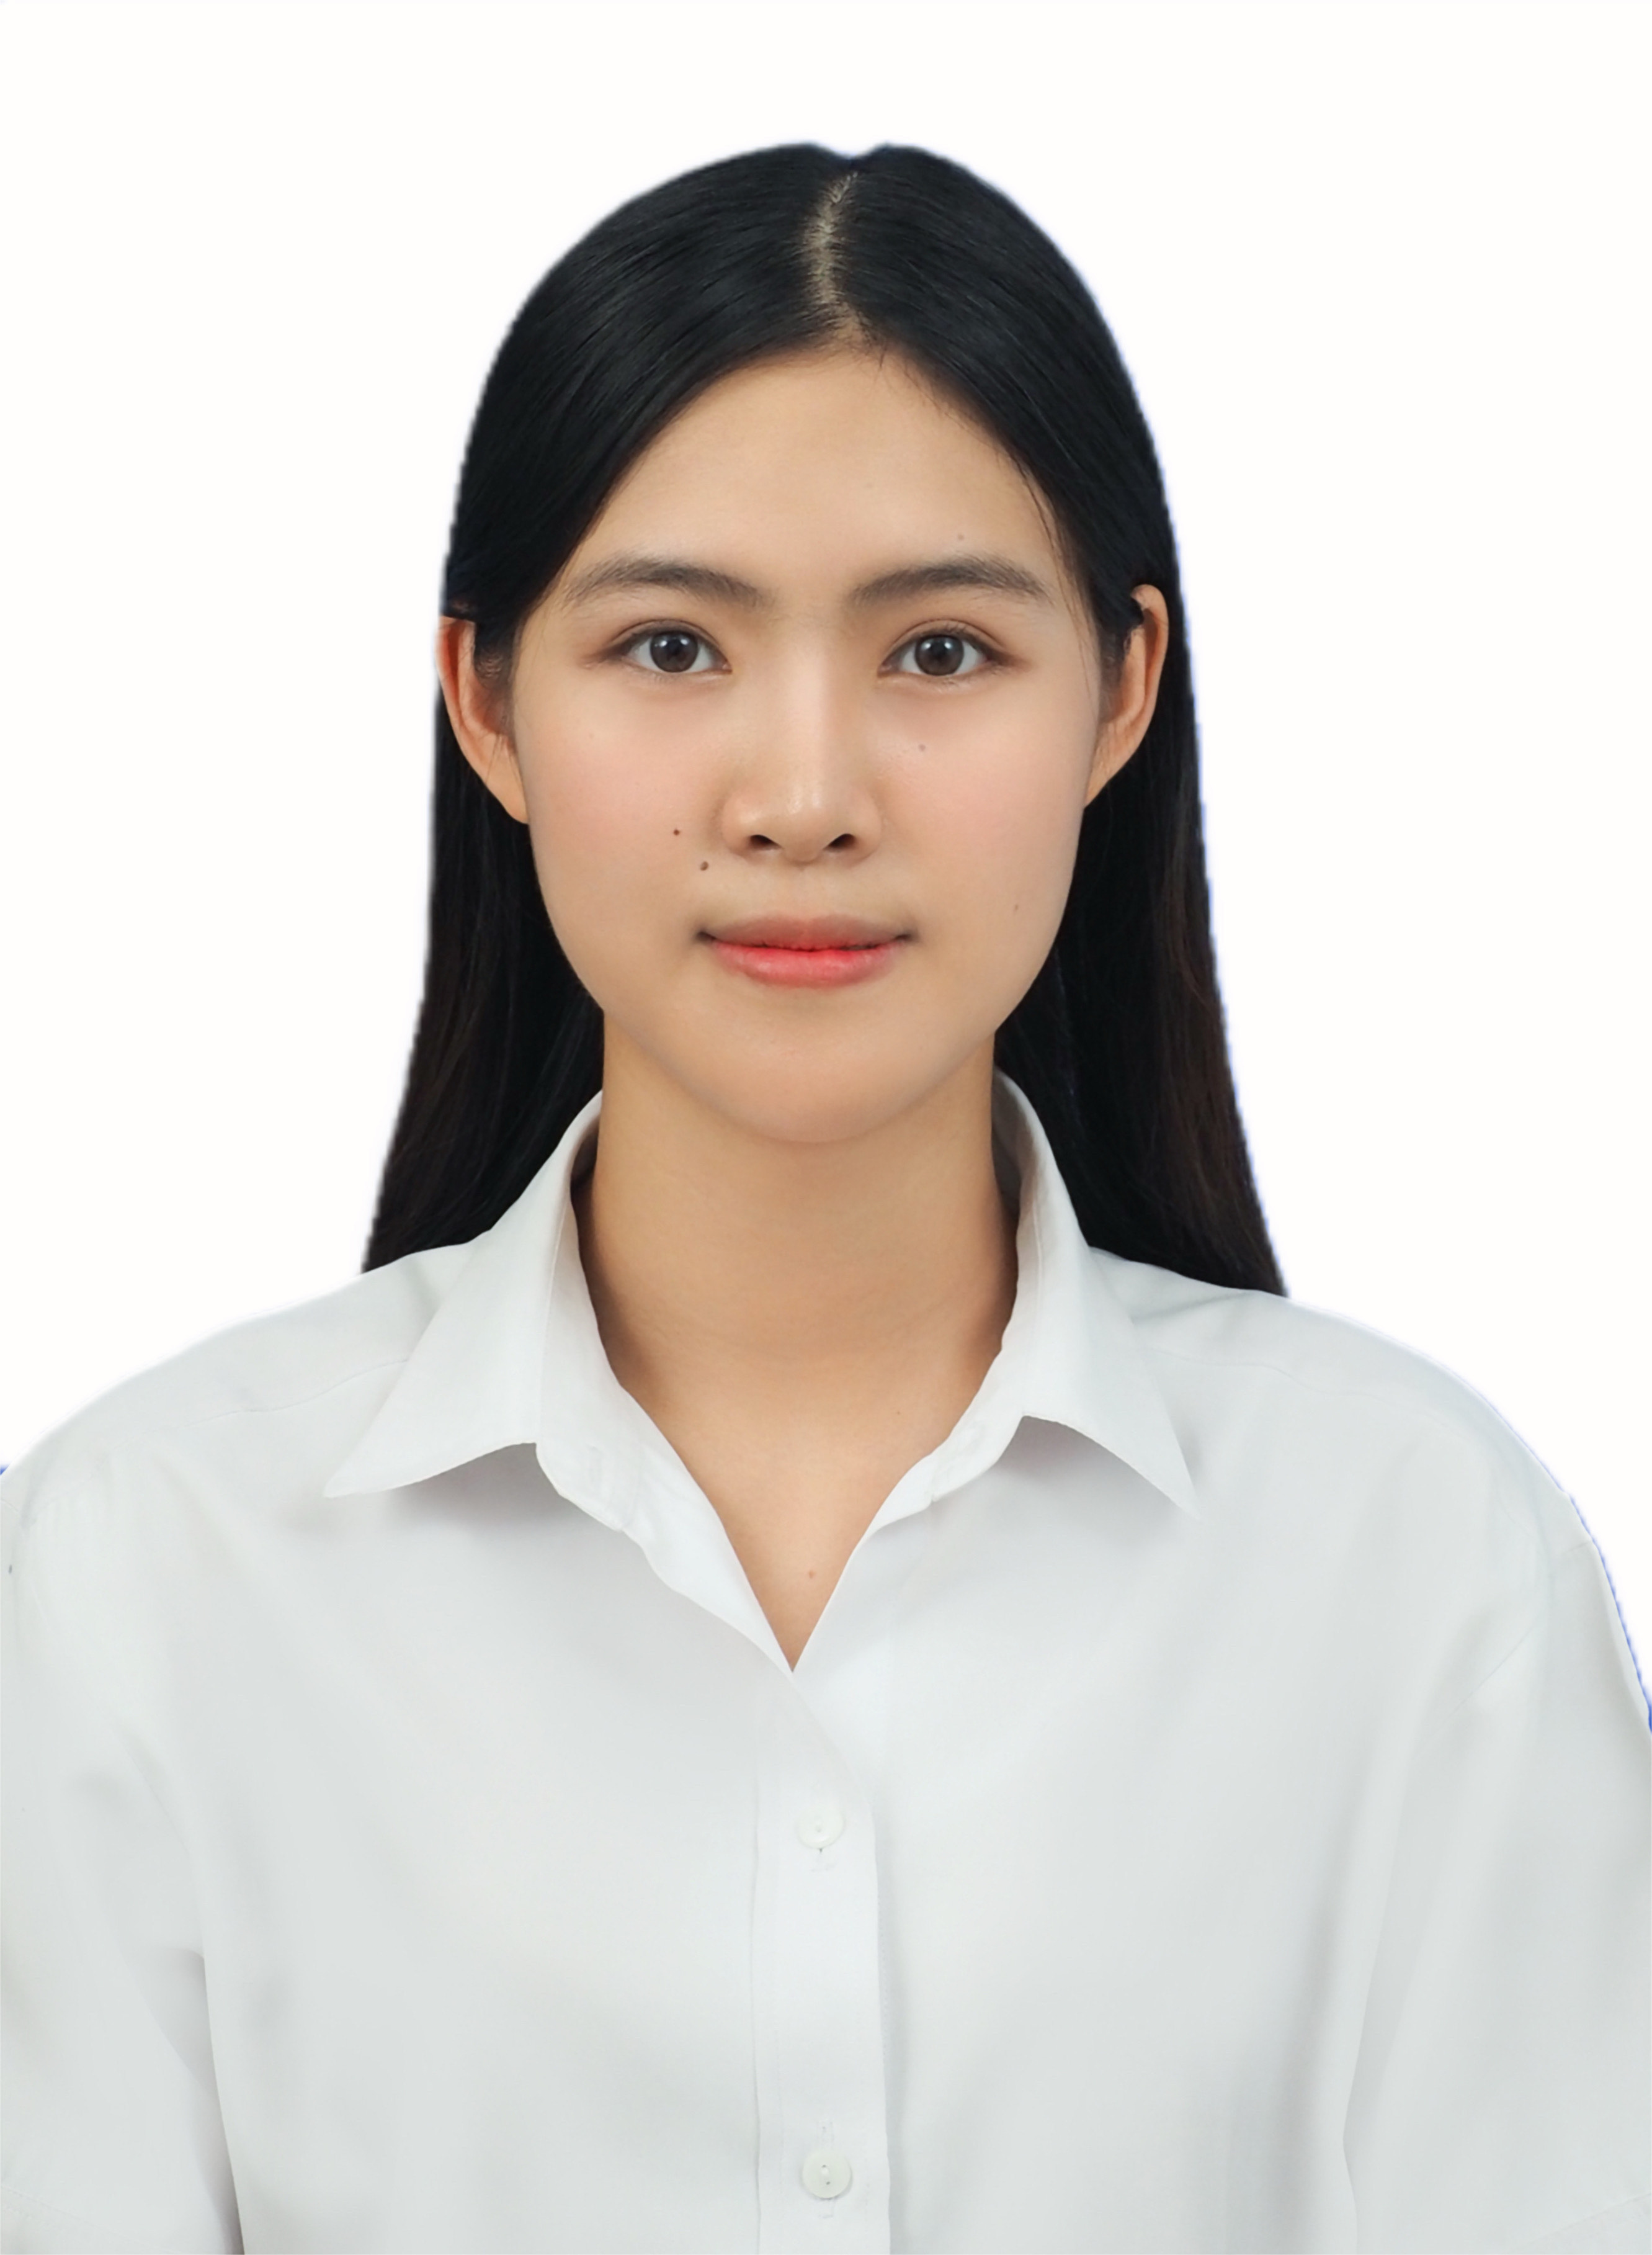
\includegraphics[width=1.5in]{0743.jpeg}
\end{center}
\textbf{Kanonlas Rattanapak (650610743)} เป็นนักศึกษาระดับปริญญาตรี ชั้นปีที่ 4 
ภาควิชาวิศวกรรมคอมพิวเตอร์ คณะวิศวกรรมศาสตร์ มหาวิทยาลัยเชียงใหม่
มีความสนใจด้าน \textit{Quantum Computing, Game Theory, และ Cybersecurity}
โดยเฉพาะการประยุกต์ทฤษฎีเกมควอนตัมกับการวิเคราะห์กลยุทธ์การป้องกันทางไซเบอร์
ปัจจุบันกำลังศึกษาวิจัยในหัวข้อ \textit{Quantum Volunteer's Dilemma}
เพื่อพัฒนาแบบจำลองเชิงควอนตัมสำหรับกลยุทธ์การโจมตีและการป้องกันในระบบเครือข่าย.

\begin{center}
  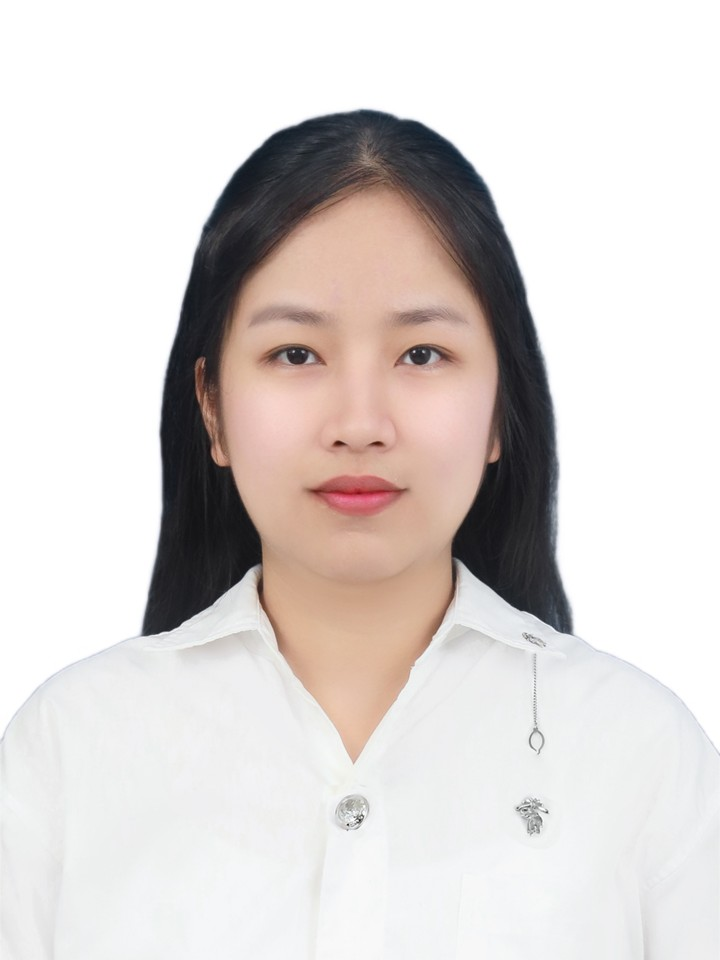
\includegraphics[width=1.5in]{0750.jpg}
\end{center}
\textbf{Kaewtar Lungta (650610750)} เป็นนักศึกษาระดับปริญญาตรี ชั้นปีที่ 4 
ภาควิชาวิศวกรรมคอมพิวเตอร์ คณะวิศวกรรมศาสตร์ มหาวิทยาลัยเชียงใหม่ มีความสนใจเฉพาะทางด้าน ความมั่นคงปลอดภัยไซเบอร์ (Cybersecurity) และ คอมพิวเตอร์ควอนตัม (Quantum Computing)
โดยมุ่งมั่นที่จะพัฒนาองค์ความรู้และทักษะเพื่อเตรียมความพร้อมต่อการเปลี่ยนแปลงของเทคโนโลยีในยุคควอนตัม

\begin{center}
  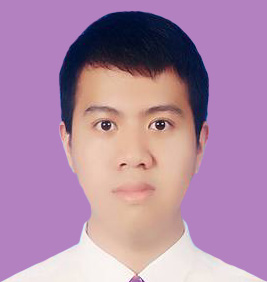
\includegraphics[width=1.5in]{0773.jpg}
\end{center}
\textbf{Theeraphan Phanwattanasin (650610773)} เป็นนักศึกษาระดับปริญญาตรี ชั้นปีที่ 4 ภาควิชาวิศวกรรมคอมพิวเตอร์ คณะวิศวกรรมศาสตร์ มหาวิทยาลัยเชียงใหม่ มีความสนใจทางด้าน Quantum Physics, Algoirthm และ Discrete Math มีความสนใจเป็นพิเศษในด้านของ การนำทฤษฎีทางคณิตศาสตร์และฟิสิกส์ ไปพัฒนาเป็นอัลกอริทึมใหม่ ๆ ในระบบควอนตัมคอมพิวเตอร์ ปัจจุบันกำลังศึกษาวิจัยในหัวข้อ Ising model และ Hamiltonian Equation เพื่อพัฒนาเป็นสมการเชิงควอนตัมในปัญหาการโจมตีและการป้องกันทางไซเบอร์
\end{biosketch}
\fi % \ifproject
\end{document}
